
\section[\textgreek{Κλειδιά}] {\textgreek {Κλειδιά σχέσεων, υπερκλειδί, υποψήφιο κλειδί, πρωτεύον κλειδί, ξένο κλειδί} }

\subsection[\textgreek{Υπερκλειδί, υποψήφιο κλειδί, πρωτεύον κλειδί}] {\textgreek {Υπερκλειδί, υποψήφιο κλειδί, πρωτεύον κλειδί} }

\begin{frame}[t, fragile]
\frametitle{Υπερκλειδί}
\begin{minipage}{0.94\textwidth}
  \large
  \begin{block}{Υπερκλειδί}
    {\bb Υπερκλειδί} ενός σχήματος μιας σχέσης $R$ αποτελεί κάθε υποσύνολο 
    γνωρισμάτων του σχήματος που, για οποιοδήποτε στιγμιότυπο $r$ της σχέσης $R$, 
    δεν υπάρχουν δύο πλειάδες με ίδιες τιμές
    στα γνωρίσματα αυτά. Δηλαδή ισχύει: \[ t_1[S] \neq t_2[S] \]
    όπου $S$ είναι υποσύνολο των γνωρισμάτων του σχήματος της $R$:
    \[ S \subseteq R \]  
  \end{block}
\end{minipage}
\end{frame}


\begin{frame}[t, fragile]
\frametitle{Παράδειγμα υπερκλειδιού}
\begin{minipage}{0.94\textwidth}
  \large
  \begin{exampleblock}{Παράδειγμα σχέσης «Φοιτητής»}
        \begin{tabular}{ c l l } \hline
        {\bf ΑρΜητ}      & {\bf Όνομα} & {\bf Επώνυμο} \\ \hline
        53  &  Μαρία     & Στεργίου  \\
        56  &  Βασιλική  & Παυλίδου  \\
        57  &  Ανίτα     & Καραβία  \\
        58  &  Πέτρος    & Τσακιρόγλου  \\ \hline
      \end{tabular} \\
      \par \bigskip
       Οι συνδυασμοί (ΑρΜητ), (ΑρΜητ, Όνομα), (ΑρΜητ, Όνομα, Επώνυμο) είναι {\cee υπερκλειδιά}
  \end{exampleblock}
\end{minipage}
\end{frame}


\begin{frame}[t, fragile]
\frametitle{Κλειδί} 
\begin{minipage}{0.94\textwidth}
  \large
  \begin{block}{Κλειδί}
    {\bb Κλειδί} ενός σχήματος μιας σχέσης $r(R)$ είναι ένα υποσύνολο των γνωρισμάτων της $R$ που είναι
    υπερκλειδί της $r(R)$, χωρίς να είναι δυνατό να αφαιρεθεί ένα γνώρισμα και να παραμείνει υπερκλειδί.
    Το κλειδί λέγεται και ελάχιστο υπερκλειδί. 
  \end{block}
\end{minipage}
\end{frame}


\begin{frame}[t, fragile]
\frametitle{Παράδειγμα κλειδιού}
\begin{minipage}{0.94\textwidth}
  \large
  \begin{exampleblock}{Παράδειγμα σχέσης «Φοιτητής»}
        \begin{tabular}{ c l l } \hline
        {\bf ΑρΜητ}      & {\bf Όνομα} & {\bf Επώνυμο} \\ \hline
        53  &  Μαρία     & Στεργίου  \\
        56  &  Βασιλική  & Παυλίδου  \\
        57  &  Ανίτα     & Καραβία  \\
        58  &  Πέτρος    & Τσακιρόγλου  \\ \hline
      \end{tabular} \\
      \par \bigskip
       Ο ΑρΜητ είναι {\cee κλειδί}. \\
       Ο συνδυασμός  (ΑρΜητ, Όνομα) είναι {\cee υπερκλειδί} αλλά όχι {\cee κλειδί}.
  \end{exampleblock}
\end{minipage}
\end{frame}



\begin{frame}[t, fragile]
\frametitle{Υποψήφιο κλειδί} 
\begin{minipage}{0.94\textwidth}
  \large
  \begin{block}{Υποψήφιο κλειδί}
    {\bb Υποψήφιο κλειδί} είναι κάθε κλειδί της της $R$. Γενικά, μια σχέση μπορεί να έχει περισσότερα 
    από ένα κλειδιά.
  \end{block}
\end{minipage}  
\end{frame}


\begin{frame}[t, fragile]
\frametitle{Πρωτεύον κλειδί}
\begin{minipage}{0.94\textwidth}
  \large
  \begin{block}{Πρωτεύον κλειδί}
    {\bb Πρωτεύον κλειδί} είναι το υποψήφιο κλειδί που επιλέγεται ώστε κάθε πλειάδα της σχέσης $R$ 
    να προσδιορίζεται μοναδικά με βάση την τιμή αυτού του κλειδιού. Κάθε σχέση έχει ένα
    {\cee και μόνο ένα} πρωτεύον κλειδί.
  \end{block}
  \begin{block}{Κανόνας ακεραιότητας των οντοτήτων}
    Το πρωτεύον κλειδί δεν μπορεί να πάρει την τιμή \tnull.
  \end{block}  
\end{minipage} 
\end{frame}



\begin{frame}[t, fragile, shrink]
\frametitle{Περισσότερα από ένα κλειδιά}
Έστω μια σχέση $r$ με σχήμα $R = \{ \alpha, \beta, \gamma, \delta\}$.
Έστω επίσης τα γνωρίσματα $\alpha$ και $\beta$ παίρνουν μοναδικές τιμές και
μπορούν να χρησιμοποιηθούν (το καθένα χωριστά) ως αναγνωριστικό (κλειδί).
\begin{minipage}{0.94\textwidth}
Τα υπερκλειδιά της σχέσης $r(R)$:
%\begin{figure}[h]
  \begin{align*}
    \{\alpha\} & & \{\beta\} & & \{\alpha, \beta\} \\
    \{\alpha, \gamma\} & & \{\alpha, \delta\} & & \{\alpha, \gamma, \delta\} \\
    \{\beta, \gamma\} & & \{\beta, \delta\} & & \{\beta, \gamma, \delta\}   \\
    \{\alpha, \beta, \gamma\} & & \{\alpha, \beta, \delta\} & & \{\alpha, \beta, \gamma, \delta\}
  \end{align*}
%\label{superkey}
%\end{figure}

Με την έννοια υπερκλειδί εννοείται κάθε σύνολο γνωρισμάτων της $r$, δηλαδή κάθε
υποσύνολο του $R$, που μπορεί να προσδιορίσει μοναδικά κάθε εγγραφή της $r$.
\end{minipage}
\end{frame}


\begin{frame}
\frametitle{Περισσότερα από ένα κλειδιά}
\begin{minipage}{0.94\textwidth}
Το παρακάτω σχήμα που δείχνει του υπαλλήλους
μιας εταιρείας.
Τόσο το ΑΦΜ (αριθμός φορολογικού μητρώου) όσο και ο ΑΜΚΑ
μπορούν να χρησιμοποιηθούν ως κλειδιά.
\begin{figure}[h]
  \begin{tabular}{ l l l l } \toprule
    {\bf ΑΦΜ} & {\bf ΑΜΚΑ} & {\bf Επώνυμο} & {\bf Όνομα} \\ \midrule
    903410281 & 4033781 & Βασιλειάδης & Αριστομένης \\
    345801248 & 7394873 & Νικολάου & Βασιλική \\
    673018337 & 7294091 & Δημητριάδης & Ιωάννης \\
    648201938 & 6483842 & Βώρος & Χαράλαμπος \\
    759120484 & 0284938 & Μακρής & Ιωάννης \\ \bottomrule
  \end{tabular}
\end{figure}
\end{minipage}
\end{frame}



\begin{frame}[t, fragile]
\frametitle{Υπογράμμιση και δήλωση πρωτεύοντος κλειδιού}
\begin{minipage}{0.94\textwidth}
  \begin{exampleblock}{Το πρωτεύον κλειδί μιας σχέσης δηλώνεται συνήθως με υπογράμμιση των γνωρισμάτων που το συνιστούν:}
    \begin{itemize}
      \item Μαθήματα (\underline{Κωδικός}, Όνομα, Εξάμηνο)
      \item Φοιτητές (\underline{ΑΜ}, Όνομα, Επώνυμο))   
      \item Αίθουσες (\underline{Κωδικός}, Όνομα, Τόπος, Χωρητικότητα)
    \end{itemize}
  \end{exampleblock}
  %
  \begin{exampleblock}{Άλλος τρόπος είναι η τοποθέτηση της δίεσης:}
    \begin{itemize}
      \item Μαθήματα (Κωδικός$\#$, Όνομα, Εξάμηνο)
      \item Φοιτητές (ΑΜ$\#$, Όνομα, Επώνυμο))   
      \item Αίθουσες (\underline{Κωδικός}, Όνομα, Τόπος, Χωρητικότητα)
    \end{itemize} 
  \end{exampleblock}
\end{minipage} 
\end{frame}


\begin{frame}[t, fragile]
\frametitle{Απλό και σύνθετο κλειδί}
\begin{minipage}{0.94\textwidth}
  \begin{block}{Το πρωτεύον κλειδί μπορεί να αποτελείται από ένα μόνο γνώρισμα:}
    \begin{itemize}
      \item Μαθήματα (\underline{Κωδικός}, Όνομα, Εξάμηνο)
      \item Φοιτητές (\underline{ΑΜ}, Όνομα, Επώνυμο))   
    \end{itemize}
    οπότε λέγεται {\bf\color{red}απλό}.
  \end{block}
  %
  \begin{block}{Ή να αποτελείται από συνδυασμό περισσότερων γνωρισμάτων:}
    \begin{itemize}
      \item Διδασκαλία (\underline{ΚωδΜαθ}, \underline{ΚωδΚαθ}, \underline{Έτος})
      \item Παραγγελίες (\underline{ΚωδΠελ}, \underline{ΚωδΠρο}, Ποσότητα)   
    \end{itemize} 
        οπότε λέγεται {\bf\color{red}σύνθετο}.
  \end{block}
\end{minipage} 
\end{frame}


\begin{frame}[t, fragile, shrink]
\frametitle{Μοναδικότητα σύνθετου κλειδιού}
\begin{minipage}{0.94\textwidth}
  \begin{columns}[T]
    \begin{column}{0.5\textwidth}
      Έστω η σχέση Διδασκαλία με σύνθετο πρωτεύον κλειδί που αποτελείται από 3 γνωρίσματα για την καταγραφή του
      ιστορικού διδασκαλίας σε ένα τμήμα. 
    \end{column}
    \begin{column}{0.5\textwidth}
      \begin{tabular}{c c c} \toprule
        {\bf ΚωδΜαθ} & {\bf ΚωδΚαθ} & {\bf Έτος} \\ \midrule
        107 & 13 & 2009 \\ 
        303 & 11 & 2009 \\
        107 & 19 & 2010 \\
        303 & 17 & 2010 \\
        508 & 17 & 2010 \\    \bottomrule
      \end{tabular}      
    \end{column}  
  \end{columns}
  \begin{block}{Μοναδικότητα}
    \begin{itemize}
      \item Ο συνδυασμός (ΚωδΜαθ, ΚωδΚαθ, Έτος) παίρνει μοναδικές τιμές.
      \item Τα γνωρίσματα ΚωδΜαθ, ΚωδΚαθ, Έτος μπορεί να πάρουν διπλότυπα, πχ ο καθηγητής με κωδικό 17.
      \item Άλλοι συνδυασμοί μπορεί να πάρουν διπλότυπα, πχ ο συνδυασμός (17,2010) για τον καθηγητή και το έτος.
    \end{itemize}
  \end{block}
  
\end{minipage} 
\end{frame}




\subsection[\textgreek{Ξένο κλειδί}] {\textgreek {Ξένο κλειδιά και σχεσιακό μοντέλο} }


\begin{frame}[t, fragile]
\frametitle{Ξένο κλειδί}
\begin{minipage}{0.94\textwidth}
  \begin{block}{Ξένο κλειδί}
    {\bb Ξένο κλειδί} είναι το πρωτεύον κλειδί μιας σχέσης $R$ που τοποθετείται ως επιπλέον γνώρισμα
    σε μια σχέση $S$, έτσι ώστε οι πλειάδες της των σχέσεων $R,S$ να συσχετίζονται μεταξύ τους.
  \end{block}
  \begin{exampleblock}{Ξένο κλειδί}
    \[
      R(\underline{A_1}, A_2, A_3) \quad \quad S(\underline{B_1}, B_2, A_1) 
    \]
    Το γνώρισμα $S.A_1$ είναι ξένο κλειδί, δεν παίρνει αναγκαστικά μοναδικές τιμές, δεν είναι πρωτεύον κλειδί
    της σχέσης $S$.
  \end{exampleblock} 
\end{minipage} 
\end{frame}


\begin{frame}[t, fragile]
\frametitle{Παράδειγμα ξένου κλειδιού, παραγγελίες}
\begin{minipage}{0.94\textwidth}
      \begin{tabular}{ c l } \hline
        {\bf ΚωδΠελ} & {\bf Όνομα}  \\ \hline 
        \rowcolor{blue!50}   1 & Νίκος     \\ 
        \rowcolor{red!50}    2 & Κατερίνα  \\
        \rowcolor{green!50}  3 & Μαριάνθη  \\ 
        \rowcolor{yellow!50} 4 & Ιωάννα    \\  \hline
      \end{tabular}
\hspace*{1cm}
      \begin{tabular}{ c r c  } \hline 
        {\bf ΑρΠαρ}  & {\bf Αξία} & {\bf ΚωδΠελ} \\ \hline 
        \rowcolor{red!50}    1  &  29.10  & 2  \\ 
        \rowcolor{blue!50}   2  &  14.00  & 1  \\ 
        \rowcolor{red!50}    3  &  10.50  & 2  \\ 
        \rowcolor{blue!50}   4  &  19.30  & 1  \\ 
        \rowcolor{yellow!50} 5  &  25.90  & 4  \\
        \rowcolor{red!50}    6  &  17.50  & 2  \\ \hline 
      \end{tabular}
\end{minipage} 
\end{frame}


\begin{frame}[t, fragile, shrink]
\frametitle{Ξένα κλειδιά, αποτελέσματα εξεταστικής}
\begin{minipage}{0.94\textwidth}

      \begin{tabular}{ c l } \hline 
        {\bf ΚωδΜαθ} & {\bf Όνομα}  \\ \hline 
         203 & Στατιστική {\en II}  \\ 
         201 & Οικονομική {\en II}  \\
         207 & Ηλεκ.Υπολ. {\en II}  \\ 
         204 & Μαθηματικά {\en II}  \\  \hline
      \end{tabular} \hspace*{0.3cm}
      \begin{tabular}{ c l l } \hline 
        {\bf ΑρΜητ}       & {\bf Όνομα} & {\bf Επώνυμο} \\ \hline 
        53  &  Μαρία     & Στεργίου  \\ 
        56  &  Βασιλική  & Παυλίδου  \\ 
        57  &  Ανίτα    & Καραβία  \\ 
        58  &  Πέτρος    & Τσακιρόγλου  \\ \hline 
      \end{tabular}
\\
\par
\vspace*{1cm}
      \begin{tabular}{ c c } \hline 
        {\bf ΑρΜητ} & {\bf Βαθμός}  \\ \hline 
         53 & 9  \\ 
         56 & 7  \\
         57 & 10  \\ 
         58 & 7  \\  \hline
      \end{tabular}  \hspace*{0.5cm}
      \begin{tabular}{ c c } \hline 
        {\bf ΚωδΜαθ}      & {\bf Βαθμός} \\ \hline 
        201  &  10  \\ 
        203  &  6  \\ 
        204  &  8  \\ 
        207  &  9  \\ \hline 
      \end{tabular}
\end{minipage} 
\end{frame}


\begin{frame}[t, fragile]
\frametitle{Αναφορική ακεραιότητα}
\begin{minipage}{0.94\textwidth}
  \begin{block}{Κανόνας ακεραιότητας των αναφορών}
    Έστω $s.A_1$ το ξένο κλειδί της σχέσης $r$ που αναφέρεται στο πρωτεύον κλειδί
    της σχέσης $r.A_1$.
    \begin{enumerate}
      \item Κάθε τιμή του ξένου κλειδιού υπάρχει ως τιμή του πρωτεύοντος κλειδιού
            στο οποίο αναφέρεται. \\
            Για παράδειγμα:
            \[ s.A_1 = r.A_1\]
      \item Η τιμή του ξένου κλειδιού δεν μπορεί να είναι \tnull.      
    \end{enumerate}
  \end{block} 
\end{minipage} 
\end{frame}


\begin{frame}[t, fragile, shrink]
\frametitle{Βέλη στα ξένα κλειδιά}
\begin{minipage}{0.94\textwidth}
        \noindent
        \tikzset{
            text depth=0ex,
            text height=1ex,
            inner sep=0pt,
        }%
    Μαθήματα   ( \tikz[remember picture]\node (id1) {\underline{Κωδικός}};, 
                 \tikz[remember picture]\node (1r2) {Όνομα};, 
                 \tikz[remember picture]\node (1r3) {Εξάμηνο};
               )\\[.5cm]
    Καθηγητές  ( \tikz[remember picture]\node (id2) {\underline{Κωδικός}};,                  
                      Όνομα, Επώνυμο, {\en E-mail})\\[.5cm]
    Διδασκαλία ( \tikz[remember picture]\node (tid1) {\underline{ΚωδΜαθ}};,
                 \tikz[remember picture]\node (tid2) {\underline{ΚωδΚαθ}};
               )   
    \begin{tikzpicture}[overlay, remember picture]
        \path[draw,thick,-latex] (id1.south) ++(0,-.1) -- ++(0,-.2) -- ++(7,0) -- ++(0,-.97) -| ($(tid1.60) + (0,.1)$);
        \path[draw,thick,-latex] (id2.south) ++(0,-.1) -- ++(0,-.2) -| ($(tid2.120) + (0,.1)$);
    \end{tikzpicture}
    
    \begin{exampleblock}{Παράδειγμα}
      \begin{itemize}
        \item Μαθήματα.Κωδικός $\rightarrow$ Διδασκαλία.ΚωδΜαθ \\
              σημαίνει πως το γνώρισμα ΚωδΜαθ της σχέσης Διδασκαλία είναι ξένο κλειδί και αναφέρεται
              στο γνώρισμα Κωδικός της σχέσης Μαθήματα.
        \item Καθηγητές.Κωδικός $\rightarrow$ Διδασκαλία.ΚωδΚαθ \\
              σημαίνει πως το γνώρισμα ΚωδΚαθ της σχέσης Διδασκαλία είναι ξένο κλειδί και αναφέρεται
              στο γνώρισμα Κωδικός της σχέσης Καθηγητές.              
      \end{itemize}
    \end{exampleblock}

\end{minipage} 
\end{frame}    

\begin{frame}
\frametitle{Γραφική αναπαράσταση σχεσιακού μοντέλου}
\begin{minipage}{\wE}
  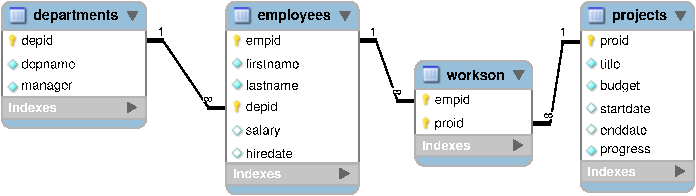
\includegraphics[scale=0.45]{../common/companyREL.pdf} \\
  \bigskip
  \par Το παράδειγμα μιας μικρής σχεσιακής βάσης δεδομένων \\ 
       για τους υπαλλήλους μιας εταιρίας και τα έργα \\
       στα οποία απασχολούνται.
\end{minipage}        
\end{frame}
